%REPORT TEMPLATE
%AUTHOR: RUI QU  
%EMAIL: RQU@KTH.SE 

%----------------------------------------------------------------------------------------
%	PACKAGES AND DOCUMENT CONFIGURATIONS
%----------------------------------------------------------------------------------------

\documentclass{article}

%---Basic---
\usepackage{natbib} % Required to change bibliography style to APA
\usepackage{amsmath} % Required for some math elements 
\setlength\parindent{0pt} % Removes all indentation from paragraphs
\usepackage{listings}%Insert code
\usepackage{times} % Uncomment to use the Times New Roman font

%---Table---
\usepackage{multirow}%Table
\usepackage{booktabs}%Table Triple-lines
\usepackage{siunitx} % Provides the \SI{}{} and \si{} command for typesetting SI units

%---Figure---
\usepackage{graphicx} % Required for the inclusion of images
\usepackage{subfigure} % Required for multiple images
\usepackage{float} 

%---Pseudo-code in LaTeX---
\usepackage{minted} %Preference->engine->pdfTeX->Latex  ADD: -shell-escape
\usepackage{xcolor}
\definecolor{bg}{rgb}{0.95,0.95,0.95}

\usepackage{algorithm}
\usepackage{algpseudocode}
\usepackage{amsmath}
\renewcommand{\algorithmicrequire}{\textbf{Input:}}  % Use Input in the format of Algorithm
\renewcommand{\algorithmicensure}{\textbf{Output:}} % Use Output in the format of Algorithm

%---Appendix---
\usepackage{appendix}
\newcommand{\upcite}[1]{\textsuperscript{\textsuperscript{\cite{#1}}}} %Upcite

%----------------------------------------------------------------------------------------
%	DOCUMENT INFORMATION
%----------------------------------------------------------------------------------------

\begin{document}

\title{CS-E5710 Bayesian Data Analysis\\Assignment 8 }                  
%\author{Rui Qu\\rui.qu@aalto.fi}
\maketitle

% If you wish to include an abstract, uncomment the lines below
% \begin{abstract}
% Abstract text
% \end{abstract}

%----------------------------------------------------------------------------------------
%	SECTION 1
%----------------------------------------------------------------------------------------

\textbf{NB} Source code is given in the Appendix.

\section{Pooled Model}
\textbf{Pystan outcome}
\begin{minted}[bgcolor=bg, linenos, fontsize=\footnotesize]{bash}
              mean se_mean     sd   2.5%    25%    50%    75%  97.5%  n_eff   Rhat
mu           92.97    0.07   3.44  86.19  90.68  92.92  95.33  99.46   2208    1.0
sigma        18.88    0.05   2.63  14.57   17.0  18.59  20.46  24.83   2387    1.0
ypred6       93.26    0.32  19.46   54.8  80.29  93.02 106.05 133.17   3727    1.0
log_lik[1]   -4.01  3.1e-3   0.14  -4.29  -4.11  -4.01  -3.92  -3.75   2029    1.0
log_lik[2]   -4.72  5.1e-3   0.26  -5.29  -4.87  -4.69  -4.53   -4.3   2487    1.0
log_lik[3]   -3.96  3.0e-3   0.14  -4.25  -4.05  -3.95  -3.86   -3.7   2218    1.0
log_lik[4]   -4.08  3.1e-3   0.15  -4.39  -4.17  -4.07  -3.97  -3.81   2251    1.0
log_lik[5]   -4.16  3.2e-3   0.15  -4.47  -4.26  -4.15  -4.05  -3.89   2268    1.0
log_lik[6]   -5.79    0.01   0.53   -7.0   -6.1  -5.72   -5.4  -4.93   2563    1.0
log_lik[7]   -3.87  3.0e-3   0.14  -4.15  -3.96  -3.86  -3.77  -3.61   2135    1.0
log_lik[8]   -4.24  3.5e-3   0.17   -4.6  -4.35  -4.24  -4.12  -3.95   2322    1.0
log_lik[9]   -3.86  3.0e-3   0.14  -4.15  -3.96  -3.86  -3.77  -3.61   2139    1.0
log_lik[10]  -4.87  5.8e-3   0.29  -5.52  -5.04  -4.83  -4.66   -4.4   2514    1.0
log_lik[11]  -3.89  3.0e-3   0.14  -4.18  -3.98  -3.88  -3.79  -3.63   2150    1.0
log_lik[12]  -3.87  3.0e-3   0.14  -4.15  -3.96  -3.86  -3.77  -3.61   2135    1.0
log_lik[13]  -3.87  3.0e-3   0.14  -4.15  -3.96  -3.86  -3.77  -3.61   2135    1.0
log_lik[14]  -4.52  4.3e-3   0.21  -4.98  -4.65   -4.5  -4.37  -4.16   2433    1.0
log_lik[15]  -3.87  3.0e-3   0.14  -4.15  -3.96  -3.86  -3.77  -3.61   2135    1.0
log_lik[16]  -4.65  4.9e-3   0.24  -5.18  -4.79  -4.62  -4.48  -4.25   2470    1.0
log_lik[17]  -4.01  3.0e-3   0.14  -4.31   -4.1  -4.01  -3.91  -3.75   2230    1.0
log_lik[18]  -4.04  3.1e-3   0.15  -4.35  -4.14  -4.04  -3.94  -3.78   2239    1.0
log_lik[19]  -7.14    0.02    0.9  -9.15  -7.67  -7.06  -6.49  -5.68   2579    1.0
log_lik[20]  -4.04  3.1e-3   0.15  -4.35  -4.14  -4.04  -3.94  -3.78   2239    1.0
log_lik[21]  -3.94  3.0e-3   0.14  -4.21  -4.03  -3.93  -3.84  -3.68   2046    1.0
log_lik[22]  -3.98  3.0e-3   0.14  -4.28  -4.07  -3.98  -3.89  -3.73   2223    1.0
log_lik[23]  -4.16  3.2e-3   0.15  -4.47  -4.26  -4.15  -4.05  -3.89   2268    1.0
log_lik[24]  -4.24  3.4e-3   0.16  -4.59  -4.35  -4.23  -4.13  -3.96   2315    1.0
log_lik[25]  -4.87  5.9e-3    0.3  -5.53  -5.04  -4.83  -4.66  -4.39   2506    1.0
log_lik[26]  -3.92  3.0e-3   0.14  -4.19  -4.01  -3.92  -3.82  -3.66   2061    1.0
log_lik[27]  -4.87  5.9e-3    0.3  -5.53  -5.04  -4.83  -4.66  -4.39   2506    1.0
log_lik[28]  -4.65  4.9e-3   0.24  -5.18  -4.79  -4.62  -4.48  -4.25   2470    1.0
log_lik[29]  -3.87  3.0e-3   0.14  -4.15  -3.96  -3.86  -3.77  -3.61   2135    1.0
log_lik[30]  -3.94  3.0e-3   0.14  -4.23  -4.03  -3.93  -3.84  -3.68   2212    1.0
lp__        -99.36    0.02   0.99 -102.1 -99.77 -99.07 -98.63 -98.35   1825    1.0
\end{minted}

\begin{minted}[bgcolor=bg, linenos, fontsize=\footnotesize]{bash}
PSIS-LOO:  -130.99351268833743
p_eff:  2.0472676065418227
\end{minted}
 
 

\begin{figure}[H]
\centering  
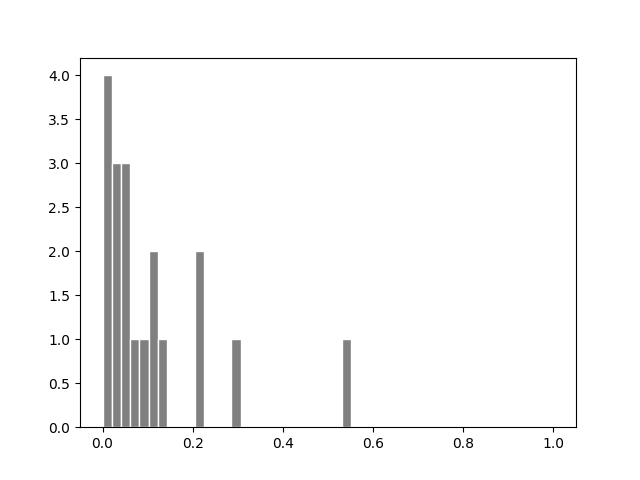
\includegraphics[scale=0.5]{pooled_hist.png}
\caption{k-values for pooled model}
\label{fig: label}
\end{figure}
For the pooled model, all the machines are considered as an entity, thus all the measurements are combined into one and performed prediction on the whole data. $\mu$ will be the same for all the machines.

\section{Separate Model}

\textbf{Pystan outcome}s
\begin{minted}[bgcolor=bg, linenos, fontsize=\footnotesize]{bash}
              mean se_mean     sd   2.5%    25%    50%    75%  97.5%  n_eff   Rhat
mu[1]        76.27    0.47  16.18  45.81  68.51  76.12  83.74 109.77   1184    1.0
mu[2]       106.43    0.34  10.13  85.72 101.78 106.36 111.04 126.63    910    1.0
mu[3]        87.18    0.36  11.58  62.81  82.48  87.57  92.73 107.66   1017    1.0
mu[4]       111.99    0.14   5.61 101.39 108.96  111.8 114.74 124.08   1709    1.0
mu[5]        89.95    0.24   9.03  71.83  85.69  89.95  94.35 108.34   1449    1.0
mu[6]        86.71    0.74  18.95  53.44  79.05  86.14  93.58 120.44    662    1.0
sigma[1]      31.3     0.7   25.1  12.54  19.02  24.99  35.71  84.27   1287    1.0
sigma[2]     19.16    0.42  13.89    7.7  11.73  15.46  21.66  55.06   1094   1.01
sigma[3]     20.98    0.66  19.12   8.23  12.66  16.53  23.14  61.78    841    1.0
sigma[4]     11.49    0.17   6.92   4.81   7.35   9.59  13.47   29.6   1691    1.0
sigma[5]     17.43    0.36  11.74   6.96  10.55  14.12  20.12  48.33   1093    1.0
sigma[6]     31.27     1.0  29.75  12.45  19.19  24.88  34.81  88.61    885   1.01
ypred6       87.55    0.94  47.47   11.4   68.4  86.97 105.76 168.46   2542    1.0
log_lik[1]   -4.36    0.01    0.5   -5.5  -4.65  -4.29   -4.0  -3.58   1173    1.0
log_lik[2]   -4.57    0.01   0.48  -5.65  -4.84  -4.51  -4.23   -3.8   1406    1.0
log_lik[3]   -4.57    0.01   0.48  -5.65  -4.84  -4.51  -4.23   -3.8   1406    1.0
log_lik[4]   -5.21    0.01   0.75  -7.23  -5.53  -5.06  -4.72  -4.24   3629    1.0
log_lik[5]   -4.39    0.01   0.49  -5.53  -4.67  -4.32  -4.04  -3.63   1316    1.0
log_lik[6]   -4.13    0.01   0.49  -5.26  -4.39  -4.06  -3.79  -3.37   1486    1.0
log_lik[7]   -3.85    0.02   0.51  -5.07  -4.13  -3.77  -3.49  -3.05   1062    1.0
log_lik[8]   -3.98    0.01   0.48  -5.13  -4.25  -3.91  -3.64  -3.22   1183    1.0
log_lik[9]   -3.84    0.02   0.51  -5.08  -4.13  -3.77  -3.48  -3.05   1046   1.01
log_lik[10]  -4.82    0.01    0.8  -6.99  -5.14  -4.65   -4.3   -3.8   3827    1.0
log_lik[11]  -4.31    0.01   0.51  -5.52  -4.59  -4.23  -3.95  -3.52   1805    1.0
log_lik[12]  -3.97    0.01   0.51  -5.19  -4.23   -3.9  -3.62   -3.2   1246    1.0
log_lik[13]  -3.95    0.01   0.51  -5.18  -4.21  -3.87   -3.6  -3.16   1235    1.0
log_lik[14]  -3.91    0.01   0.52  -5.17  -4.18  -3.83  -3.55  -3.11   1233    1.0
log_lik[15]  -4.88    0.01   0.79  -6.95  -5.22   -4.7  -4.35  -3.87   4528    1.0
log_lik[16]  -3.64    0.01   0.46  -4.69  -3.91  -3.58   -3.3  -2.89   2102    1.0
log_lik[17]   -3.7  9.1e-3   0.46  -4.77  -3.96  -3.65  -3.37  -2.95   2543    1.0
log_lik[18]  -3.46    0.01   0.45  -4.45  -3.73  -3.42  -3.14  -2.73   1884    1.0
log_lik[19]  -3.97  9.7e-3   0.56  -5.28  -4.26  -3.88  -3.57  -3.14   3405    1.0
log_lik[20]  -3.46    0.01   0.45  -4.45  -3.73  -3.42  -3.14  -2.73   1884    1.0
log_lik[21]  -4.14    0.01   0.51  -5.32  -4.41  -4.07  -3.77  -3.35   1766    1.0
log_lik[22]  -3.89    0.01   0.48  -5.02  -4.17  -3.82  -3.54  -3.12   1349    1.0
log_lik[23]  -4.27    0.01   0.55  -5.56  -4.57  -4.19  -3.89  -3.43   3012    1.0
log_lik[24]  -4.14    0.01   0.51  -5.32  -4.41  -4.07  -3.77  -3.35   1766    1.0
log_lik[25]  -3.75    0.02   0.51  -4.98  -4.05  -3.67  -3.37  -2.93   1151    1.0
log_lik[26]  -5.16    0.01   0.72  -7.03  -5.47   -5.0  -4.68  -4.19   3795    1.0
log_lik[27]  -4.34    0.02   0.51  -5.53  -4.62  -4.26   -4.0  -3.55    849    1.0
log_lik[28]  -4.64    0.01   0.49  -5.79   -4.9  -4.57   -4.3  -3.87   1227    1.0
log_lik[29]  -4.39    0.02    0.5  -5.59  -4.66  -4.31  -4.04  -3.61    836    1.0
log_lik[30]  -4.51    0.02   0.48  -5.65  -4.77  -4.44  -4.17  -3.77    992    1.0
lp__        -81.31    0.11   3.22 -88.76 -83.17 -80.92 -78.97 -76.26    873    1.0
\end{minted}

\begin{minted}[bgcolor=bg, linenos, fontsize=\footnotesize]{bash}  
PSIS-LOO:  -132.26760017922143
p_eff:  9.727184814117123
\end{minted}
 
 \begin{figure}[H]
\centering  
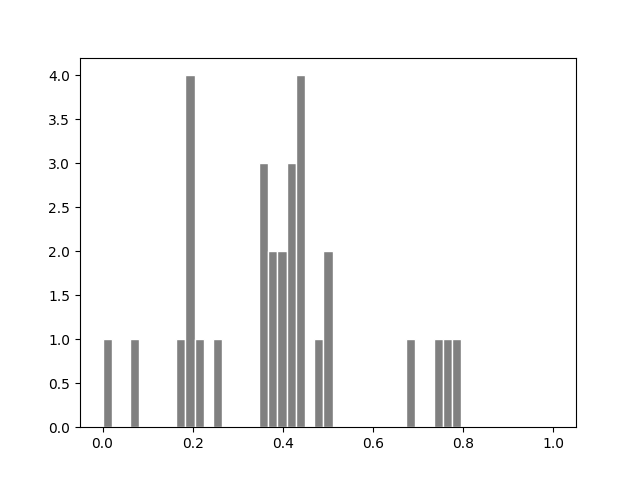
\includegraphics[scale=0.5]{separate_hist.png}
\caption{k-values for separate model}
\label{fig: label}
\end{figure}

For separate model we treat each machine separately.

\section{Hierarchical Model}
\textbf{Pystan outcome}
\begin{minted}[bgcolor=bg, linenos, fontsize=\footnotesize]{bash}
              mean se_mean     sd   2.5%    25%    50%    75%  97.5%  n_eff   Rhat
mu0          93.16     0.2    8.4   77.4  88.62  93.05  97.41 110.52   1779    1.0
sigma0       16.34    0.27  10.17   4.67  10.13  14.03  19.34  43.27   1441    1.0
mu[1]        80.13    0.19   7.06  66.12  75.51  79.99  84.87   94.3   1383    1.0
mu[2]       103.11    0.13   6.71  89.88  98.56 102.91 107.67 116.28   2524    1.0
mu[3]         89.1    0.12   6.09  77.05  85.16  89.06  93.16 101.11   2783    1.0
mu[4]       107.15    0.18   7.01  93.06 102.51 107.41 111.96 120.36   1549    1.0
mu[5]         90.7     0.1   6.15  78.45  86.67  90.73  94.71 102.88   4065    1.0
mu[6]        87.68    0.12   6.29  75.16   83.6  87.73  92.01  99.74   2651    1.0
sigma        15.32    0.05    2.4  11.45  13.64  15.02  16.67  20.77   2316    1.0
ypred6       87.45    0.25  16.09  56.09  76.53  87.13  98.02 119.33   4165    1.0
mu7           93.5    0.35  20.39  55.33  83.17  93.26 103.42 135.67   3325    1.0
log_lik[1]   -3.77  4.4e-3   0.22  -4.29  -3.88  -3.74  -3.62  -3.42   2602    1.0
log_lik[2]   -4.08  7.5e-3   0.42  -5.17  -4.26  -3.99  -3.79  -3.57   3116    1.0
log_lik[3]   -4.08  7.5e-3   0.42  -5.17  -4.26  -3.99  -3.79  -3.57   3116    1.0
log_lik[4]   -6.34    0.02   1.12  -8.81  -7.06  -6.22  -5.52  -4.51   2229    1.0
log_lik[5]   -4.11    0.01   0.42  -5.13  -4.35  -4.03   -3.8  -3.52   1002    1.0
log_lik[6]   -4.15  7.9e-3   0.41  -5.14  -4.39   -4.1  -3.84  -3.56   2716    1.0
log_lik[7]    -3.8  5.4e-3   0.25  -4.41  -3.94  -3.77  -3.63  -3.41   2074    1.0
log_lik[8]   -3.99  6.8e-3   0.34  -4.82  -4.18  -3.94  -3.74  -3.49   2498    1.0
log_lik[9]   -3.73  4.6e-3    0.2  -4.21  -3.84  -3.71   -3.6  -3.41   1865    1.0
log_lik[10]  -4.34  9.7e-3   0.52  -5.68  -4.62  -4.22  -3.96  -3.67   2930    1.0
log_lik[11]  -4.04  5.7e-3   0.35   -4.9  -4.21  -3.97   -3.8  -3.55   3674    1.0
log_lik[12]  -3.75  4.1e-3   0.21  -4.22  -3.86  -3.73  -3.61  -3.43   2461    1.0
log_lik[13]  -3.74  4.1e-3    0.2  -4.18  -3.85  -3.71   -3.6  -3.41   2283    1.0
log_lik[14]  -3.74  4.6e-3    0.2  -4.19  -3.85  -3.71   -3.6   -3.4   1909    1.0
log_lik[15]  -4.82    0.01   0.63  -6.35  -5.16  -4.72  -4.37  -3.89   3431    1.0
log_lik[16]  -3.75  4.4e-3    0.2  -4.22  -3.87  -3.73  -3.61  -3.42   2121    1.0
log_lik[17]  -4.04    0.01   0.39  -4.99  -4.25  -3.96  -3.75  -3.49   1323    1.0
log_lik[18]   -3.9  9.0e-3   0.32   -4.7  -4.07  -3.83  -3.67  -3.44   1275    1.0
log_lik[19]  -3.81  4.6e-3   0.24   -4.4  -3.92  -3.77  -3.65  -3.45   2626    1.0
log_lik[20]   -3.9  9.0e-3   0.32   -4.7  -4.07  -3.83  -3.67  -3.44   1275    1.0
log_lik[21]  -4.03  5.5e-3   0.34  -4.88   -4.2  -3.97  -3.79  -3.54   3752    1.0
log_lik[22]  -3.81  4.4e-3   0.24   -4.4  -3.93  -3.77  -3.64  -3.44   3042    1.0
log_lik[23]  -4.07  5.7e-3   0.37  -4.98  -4.24  -3.99  -3.81  -3.56   4078    1.0
log_lik[24]  -4.03  5.5e-3   0.34  -4.88   -4.2  -3.97  -3.79  -3.54   3752    1.0
log_lik[25]  -3.72  4.1e-3   0.19  -4.15  -3.83   -3.7  -3.59  -3.41   2205    1.0
log_lik[26]  -5.85    0.02   0.95  -8.01  -6.41  -5.73  -5.16  -4.37   3680    1.0
log_lik[27]  -3.77  4.2e-3   0.22  -4.29  -3.88  -3.74  -3.62  -3.43   2669    1.0
log_lik[28]  -4.34  8.5e-3    0.5   -5.6  -4.58  -4.24  -3.98  -3.68   3457    1.0
log_lik[29]  -3.97  6.6e-3   0.33  -4.75  -4.15  -3.92  -3.74  -3.49   2416    1.0
log_lik[30]  -4.08  6.4e-3   0.38  -5.07  -4.25   -4.0  -3.81  -3.57   3623    1.0
lp__        -108.9    0.07   2.56 -114.8 -110.4 -108.5 -107.0 -105.1   1209   1.01
\end{minted}

\begin{minted}[bgcolor=bg, linenos, fontsize=\footnotesize]{bash}  
PSIS-LOO:  -126.94254994864687
p_eff:  5.717938460621397
\end{minted}

\begin{figure}[H]
\centering  
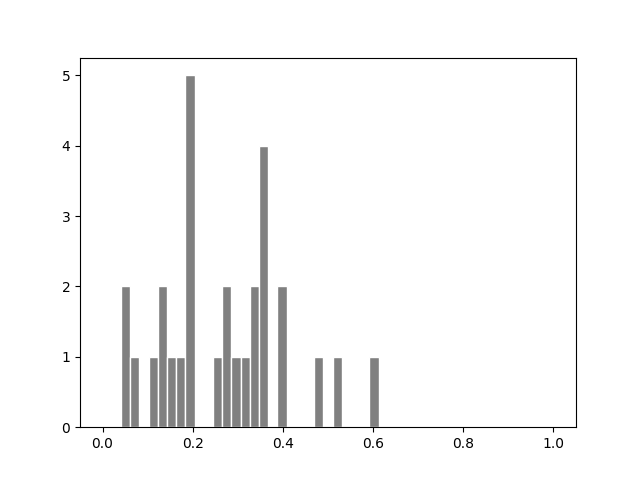
\includegraphics[scale=0.5]{hierarchical_hist.png}
\caption{k-values for hierarchical model}
\label{fig: label}
\end{figure}
The hierarchical model not only treats every machine separately, but also computes the combination of all the machines as one entity. Thus, it can predict or the machines even without data.

\begin{center}
\begin{tabular}{ccc}
	\toprule
	&PSIS-LOO&p\_eff\\
	\midrule
	Pooled Model& -130.9935&2.0473\\
	Separate Model&-132.2676&9.7272\\
	Hierarchical Model&-126.9425&5.7179\\
	\bottomrule
\end{tabular}
\end{center}

From the tabular summary above, we can see that both pooled and hierarchical models are reliable for PSIS-LOO estimations. It's because of the way how pooled and hierarchical model use the parameters. The effective number of parameters is more than 1 and less than 7 for the two models. 
\appendix
\section{Code}

\begin{minted}[bgcolor=bg, linenos, fontsize=\footnotesize]{python}  
import numpy as np
import pandas as pd
import matplotlib.pyplot as plt
from scipy.stats import norm
import pystan
import psis

machines = pd.read_fwf('./factory.txt', header=None).values
machines_transposed = machines.T

def psisloo_computation(log_lik, fig_name, model_name):
    
    #PSIS-LOO values
    psis_loo = psis.psisloo(log_lik)
    lppd_loocv = psis_loo[0]
    print('PSIS-LOO: ', lppd_loocv) 

    #The effective number of parameters
    S = np.size(log_lik, 0)
    lppd = sum(np.log([1/S*sum(np.exp(col)) for col in log_lik.T]))
    p_loocv = lppd - lppd_loocv
    print('p_eff: ', p_loocv) 
    
    #k-values visualization
    psis_hist = psis_loo[2]
    plt.hist(psis_hist, bins= np.linspace(0, 1, num=50), color='grey',ec='white')
    plt.savefig('./{0}'.format(fig_name))
    plt.show()

'''
Pooled model
'''
stan_code_pooled = '''
data {
    int<lower=0> N;       // number of data points
    vector[N] y;          //
}
parameters {
    real mu;              // group means
    real<lower=0> sigma;  // common std
}
model {
    y ~ normal(mu, sigma);
}
generated quantities {
    real ypred6;
    vector[N] log_lik;
    ypred6 = normal_rng(mu, sigma);
    for (i in 1:N)
        log_lik[i] = normal_lpdf(y[i] | mu, sigma);
}
'''
machines_pooled = machines.flatten()
model_pooled = pystan.StanModel(model_code=stan_code_pooled)
data_pooled = dict(
    N=machines_pooled.size,
    y=machines_pooled
)

fit_pooled = model_pooled.sampling(data=data_pooled)
print(fit_pooled)

log_lik_pooled = fit_pooled.extract(permuted=True)['log_lik']
psisloo_computation(log_lik_pooled, 'pooled_hist.png', 'Pool')

'''
Separate model
'''
stan_code_separate = '''
data {
    int<lower=0> N;               // number of data points
    int<lower=0> K;               // number of groups
    int<lower=1,upper=K> x[N];    // group indicator
    vector[N] y;
}
parameters {
    vector[K] mu;                 // group means
    vector<lower=0>[K] sigma;     // group stds
}
model {
    y ~ normal(mu[x], sigma[x]);
}
generated quantities {
    real ypred6;
    vector[N] log_lik;
    ypred6 = normal_rng(mu[6], sigma[6]);
    for (i in 1:N)
        log_lik[i] = normal_lpdf(y[i] | mu[x[i]], sigma[x[i]]);
}
'''

model_seperate = pystan.StanModel(model_code=stan_code_separate)
data_separate = dict(
    N=machines_transposed.size,
    K=6,
    x=[
        1, 1, 1, 1, 1,
        2, 2, 2, 2, 2,
        3, 3, 3, 3, 3,
        4, 4, 4, 4, 4,
        5, 5, 5, 5, 5,
        6, 6, 6, 6, 6,
    ],
    y=machines_transposed.flatten()
)

fit_separate = model_seperate.sampling(data=data_separate, n_jobs=-1)
print(fit_separate)

log_lik_separate = fit_separate.extract(permuted=True)['log_lik']
psisloo_computation(log_lik_separate, 'separate_hist.png', 'Separate')

'''
Hierarchical model
'''
stan_code_hierarchical = '''
data {
    int<lower=0> N;             // number of data points
    int<lower=0> K;             // number of groups
    int<lower=1,upper=K> x[N];  // group indicator
    vector[N] y;
}
parameters {
    real mu0;                   // prior mean
    real<lower=0> sigma0;       // prior std
    vector[K] mu;               // group means
    real<lower=0> sigma;        // common std
}
model {
    mu ~ normal(mu0, sigma0);
    y ~ normal(mu[x], sigma);
}
generated quantities {
    real ypred6;
    real mu7;
    vector[N] log_lik;
    ypred6 = normal_rng(mu[6], sigma);
    mu7 = normal_rng(mu0, sigma0);
    for (i in 1:N)
        log_lik[i] = normal_lpdf(y[i] | mu[x[i]], sigma);
}
'''

model_hierarchical = pystan.StanModel(model_code=stan_code_hierarchical)
data_hierarchical = dict(
    N=machines_transposed.size,
    K=6,
    x=[
        1, 1, 1, 1, 1,
        2, 2, 2, 2, 2,
        3, 3, 3, 3, 3,
        4, 4, 4, 4, 4,
        5, 5, 5, 5, 5,
        6, 6, 6, 6, 6,
    ],
    y=machines_transposed.flatten()
)
fit_hierarchical = model_hierarchical.sampling(data=data_hierarchical, n_jobs=-1)
print(fit_hierarchical)

log_lik_hierarchical = fit_hierarchical.extract(permuted=True)['log_lik']
psisloo_computation(log_lik_hierarchical, 'hierarchical_hist.png', 'hierarchical')
\end{minted}




\end{document}